\documentclass[12pt,a4paper,openright,twoside]{book}
\usepackage[utf8]{inputenc}
\usepackage{disi-thesis}
\usepackage{code-lstlistings}
\usepackage{notes}
\usepackage{shortcuts}
\usepackage{acronym}
\usepackage{float}

\school{\unibo}
\programme{Corso di Laurea in Ingegneria e Scienze Informatiche}
\title{Utilizzo di Neverlang per la modellazione di Domain Specific Languages\note{TODO: chiedere conferma titolo}}
\author{Terenzi Mirco}
\date{\today}
\subject{Programmazione ad Oggetti}
\supervisor{Prof. Viroli Mirko}
\cosupervisor{Prof. Aguzzi Gianluca}
\session{II}
\academicyear{2023-2024}

% Definition of acronyms
\acrodef{FOP}{Feature-Oriented Programming}
\acrodef{OOP}{Object-Oriented Programming}
\acrodef{DSL}{Domain-Specific Language}
\acrodef{JVM}{Java Virtual Machine}
\acrodef{AST}{Abstract Syntax Tree}
\acrodef{CFG}{Context-Free Grammar}
\acrodef{SQL}{Structured Query Language}


\mainlinespacing{1.241} % line spacing in mainmatter, comment to default (1)

\begin{document}

\frontmatter\frontispiece

\begin{abstract}    
%TODO
\end{abstract}

%----------------------------------------------------------------------------------------
\tableofcontents   
\listoffigures     % (optional) comment if empty
%\lstlistoflistings % (optional) comment if empty
%----------------------------------------------------------------------------------------

\mainmatter

%----------------------------------------------------------------------------------------
\chapter{Introduzione} %TODO
\label{chap:introduzione}
%----------------------------------------------------------------------------------------

\paragraph{Struttura della Tesi} %TODO

%----------------------------------------------------------------------------------------
\chapter{Contesto}
\label{chap:contesto}
%----------------------------------------------------------------------------------------

\section{Domain-Specific Languages}
In modo del tutto opposto rispetto ai linguaggi general-purpose, progettati per poter essere utilizzati in ogni contesto con un’efficienza e 
un grado d’espressività relativamente uguali, i \ac{DSL} sono ottimizzati per uno specifico ambito e risultano essere, in molti casi, una 
soluzione molto più naturale rispetto a quella fornita dai primi \cite{Hudak1997}. Tra gli esempi più comuni di \ac{DSL} troviamo SQL, LaTeX 
(utilizzato anche per la scrittura di questo documento) e CSS.

Nonostante la definizione di \ac{DSL} sia chiara, non è altrettanto immediato definire se un linguaggio sia o meno un \ac{DSL}. In questo caso, 
vi sono alcuni principi chiave da osservare \cite{Fowler2010}\sidenote{TODO: è corretto inserire qui il riferimento alla documentazione utilizzata per ciò che è scritto all'interno dell'elenco puntato?}:
\begin{itemize}
    \item Un \ac{DSL} è un linguaggio di programmazione e, come tale, la sua struttura dovrebbe essere progettata in modo da essere facile da 
    comprendere per gli esseri umani e, al tempo stesso, eseguibile da un calcolatore.
    \item Essendo un linguaggio, deve avere un senso di fluidità e la sua espressività deve essere derivata non solo da un’espressione 
    individuale, ma anche dalla combinazione di più istruzioni.
    \item Coerentemente alla definizione, un \ac{DSL} dovrebbe implementare l'insieme minimo di caratteristiche necessarie per poter supportare 
    il dominio applicativo di interesse ed evitare funzioni non fondamentali che potrebbero rendere il linguaggio più difficile, 
    sia da utilizzare sia da comprendere.
\end{itemize}

L’utilizzo di questa tipologia di linguaggi di programmazione comporta una serie di vantaggi:
\begin{itemize}
    \item \textbf{Produttività}: Essendo il livello d’astrazione maggiore, di conseguenza, lo è anche la produttività. Questo perché è 
    possibile utilizzare direttamente i concetti propri del dominio applicativo, non essendo limitati dalla necessità di mantenere una 
    generalità atta ad ottenere un linguaggio applicabile in molteplici contesti  \cite{Kelly2008}. Come indicato da Paul Hudak 
    \cite{Hudak1997} ed illustrato nella \cref{fig:sw-dev-cost}, assumendo che il costo di sviluppo di un programma sia lineare, possiamo 
    ipotizzare che il costo iniziale richiesto sia maggiore nel caso si utilizzasse un \ac{DSL} rispetto a metodologie più convenzionali 
    (considerando il caso in cui il linguaggio andasse sviluppato, se ne venisse utilizzato uno esistente tale costo sarebbe significativamente 
    minore). Ciò nonostante, la pendenza della curva è considerevolmente più bassa e quindi, da un determinato punto in poi, l’utilizzo di 
    \ac{DSL} porterebbe un risparmio significativo.
    \begin{figure}[H]
        \centering
        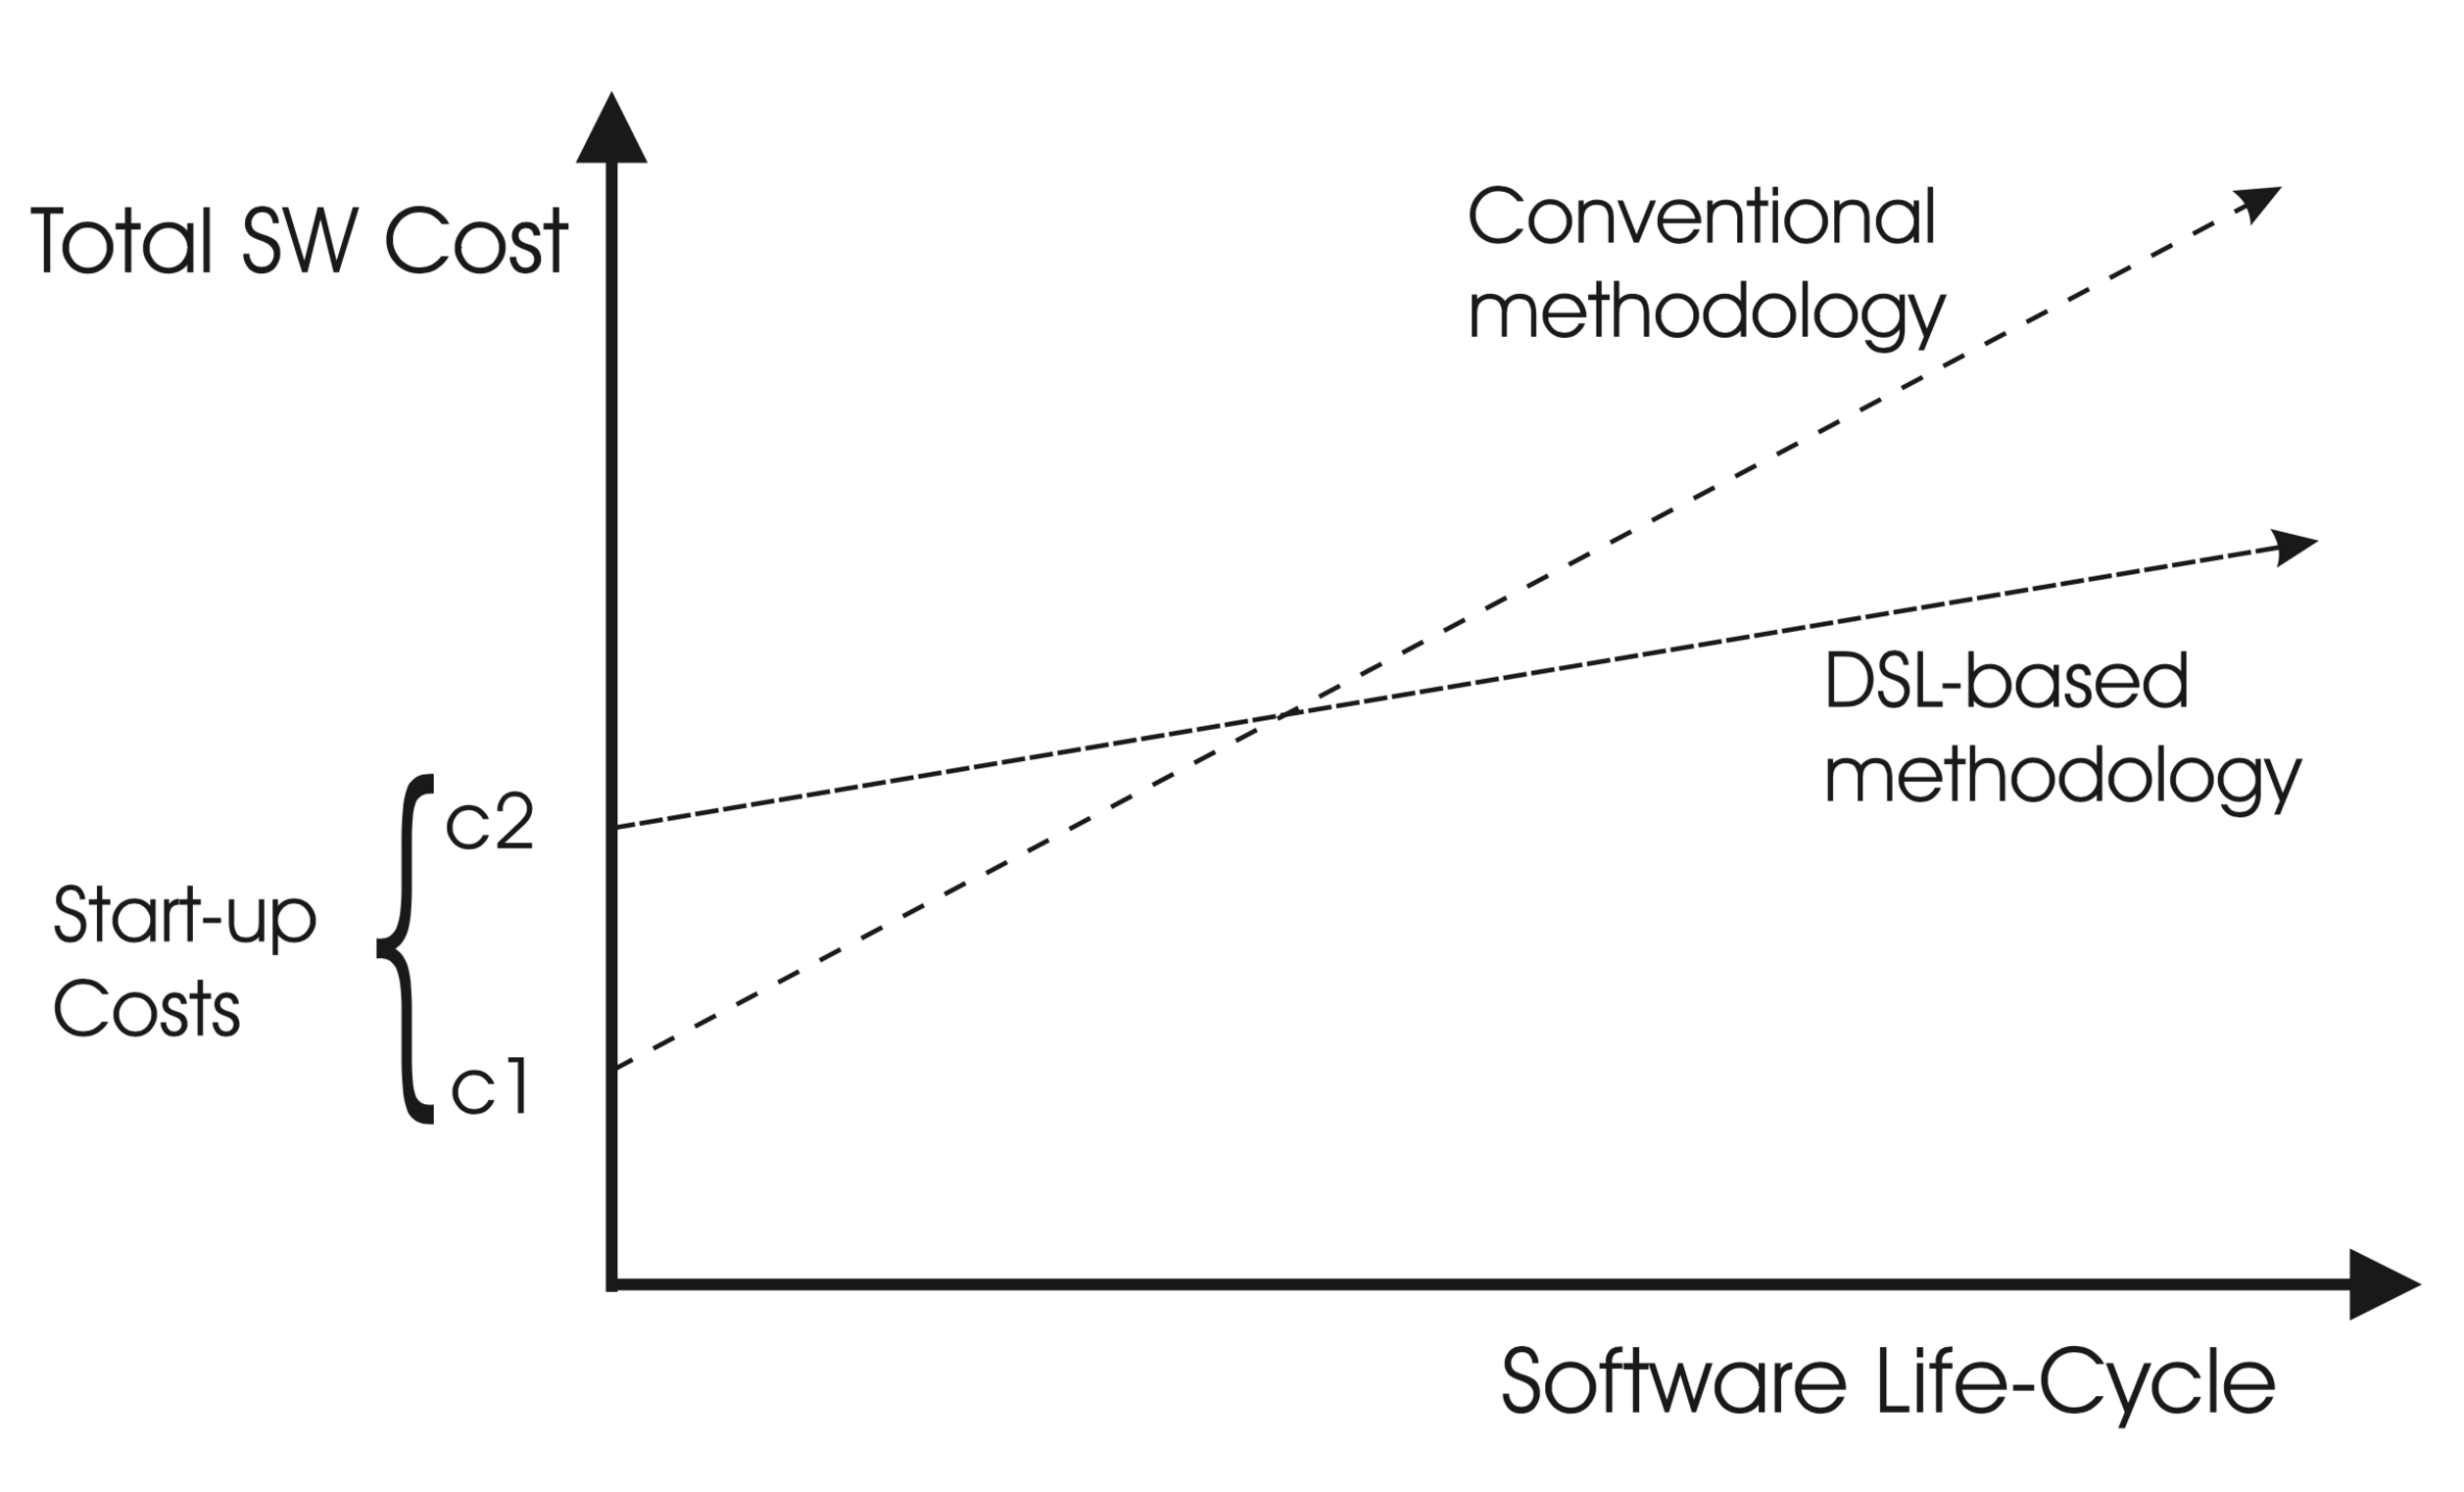
\includegraphics[width=.8\linewidth]{figures/sw-dev-cost.pdf}
        \caption{Grafico rappresentante il costo di sviluppo di un software in funzione del tempo, confrontando l'utilizzo di un DSL con 
        quello di un linguaggio general-purpose.}
        \label{fig:sw-dev-cost}
    \end{figure}
    \item \textbf{Qualità del codice}: L'utilizzo di \ac{DSL} favorisce anche una migliore qualità del codice. Infatti, il linguaggio può 
    includere regole direttamente trasposte dal dominio all'interno del quale è applicato. In questo modo risulta molto più difficile, talvolta 
    impossibile, ottenere dei risultati non attesi. Ad esempio, Antti Raunio, capo ingegnere del progetto EADS \cite{EADS}, afferma che ``la 
    qualità del codice generato è chiaramente migliore [...] perché il linguaggio di modellazione è stato progettato per adattarsi 
    all'architettura del nostro terminale''\footnote{Di seguito riportata l'affermazione citata, in lingua originale:``the quality of the 
    generated code is clearly better, simply because the modelling language was designed to fit our terminal architecture''}. Inoltre, 
    l'offuscamento della reale complessità del problema, dovuto all'utilizzo di \ac{DSL}, consente ai nuovi sviluppatori di lavorare ad un 
    alto livello d'astrazione, senza dover conoscere tutti i dettagli inerenti all'implementazione del linguaggio \cite{EADS}. 
    \item \textbf{Migliore manutenibilità}: Sebbene l'uso di \ac{DSL} non renda l'implementazione necessariamente meno complessa di quanto 
    si possa ottenere utilizzando un linguaggio \textit{general-purpose}, la manutenibilità del codice risulta essere accentuata %TODO: è corretto "accentuata"?
    \cite{Klint2010}.  Infatti, considerando il volume del codice, l'utilizzo di \ac{DSL} comporta una minor quantità di codice da comprendere, 
    facilitandone la modifica. Inoltre, è possibile  ignorare il problema di mantenere coerente ciò che è definito dalla grammatica con la 
    struttura gerarchica definita dall'\ac{AST} in quanto quest'ultimo si evolve con la prima \cite{Brabrand2010}.
\end{itemize}

\section{Grammatica non contestuale}
Nel campo dell’informatica, una grammatica formale è costituita da regole che descrivono precisamente come vengono generati i simboli di un 
linguaggio formale, partendo da un insieme finito chiamato alfabeto. Ogni regola sintattica, detta anche produzione, è espressa nella forma 
$A \rightarrow x$, dove $A$ è un simbolo non terminale e $x$ è una combinazione di simboli terminali e/o non terminali.

In particolare, la grammatica non contestuale, o \ac{CFG}, è un tipo specifico di grammatica formale che deriva il proprio nome dal fatto che 
le regole sintattiche mantengono la loro validità indipendentemente dai simboli che precedono o seguono il simbolo non terminale a cui si 
applicano. Questa caratteristica è dovuta al fatto che le regole sintattiche di una grammatica non contestuale ammettono soltanto una variabile 
non terminale sul lato sinistro della regola \cite{Linz2022}.

Le grammatiche non contestuali assumono un ruolo fondamentale nella teoria dei linguaggi formali, in particolare nella definizione e nell’analisi 
dei linguaggi di programmazione. La \ac{CFG} è utilizzata principalmente per la modellazione della sintassi, ma viene impiegata anche nella 
costruzione di interpreti e compilatori \cite{Linz2022}.

\section{Compilazione del codice}
Il compilatore è un software fondamentale nel campo della programmazione e dell’informatica, il cui compito è tradurre il codice sorgente 
(scritto in un linguaggio di alto livello) in un linguaggio di basso livello (tipicamente il linguaggio macchina o codice oggetto) che può 
essere eseguito 
dal calcolatore.

Il processo di compilazione è suddiviso in diverse fasi, ognuna delle quali ha un ruolo specifico nel convertire il codice sorgente in un 
programma eseguibile. Le fasi principali sono di seguito elencate \cite{Aho2006}:
\begin{itemize}
    \item \textbf{Analisi lessicale}: Durante la fase dell'analisi lessicale, talvolta definita anche \textit{scanning}, la sequenza di 
    caratteri di input viene analizzata e divisa in porzioni significative, chiamate lessemi. Per ogni lessema viene prodotto come output un 
    token, definito come coppia di valori \texttt{<nome-token, valore-attributo>}, che viene processato dalla fase successiva.
    \item \textbf{Analisi sintattica}: La fase dell'analisi sintattica, più comunemente indicata come \textit{parsing} (allo stesso modo, 
    il programma che svolge queste operazioni è chiamato \textit{parser}) o in italiano parsificazione, prevede che i token siano 
    utilizzati per creare una rappresentazione ad albero che descriva efficacemente la struttura grammaticale dell'input. Un esempio di 
    questo tipo di rappresentazione è costituito dall'albero sintattico. Al suo interno, ogni nodo rappresenta un'operazione e i nodi ad 
    esso discendenti, chiamati anche figli, rappresentano gli operandi dell'operazione definita dal primo. La parsificazione è svolta 
    principalmente secondo due metodologie \cite{Grune2006}:
    \begin{itemize}
        \item l’analisi \textbf{top-down} consiste nell'emulare il processo di produzione della frase. In questo modo, partendo dal simbolo 
        iniziale si procede per fasi ad evolvere l'output in modo da farlo corrispondere alla frase ottenuta come input. Il nome indica che 
        l'albero sintattico viene costruito partendo dall'alto, ossia dal nodo radice, proseguendo verso il basso;
        \item l’analisi \textbf{bottom-up}, al contrario, prevede di invertire il processo di produzione della frase, avendo come obiettivo 
        quello di ridurre la frase di input al simbolo iniziale.
    \end{itemize}
    \item \textbf{Analisi semantica}: In questo stadio della compilazione, il fine è analizzare la correttezza semantica del programma. Più 
    nello specifico, vengono utilizzati l'albero sintattico ottenuto dalla fase precedente e la tabella dei simboli per controllare che 
    l'input sia semanticamente coerente con quanto è definito dal linguaggio. Una parte fondamentale dell'analisi semantica è quella del 
    controllo del tipo (in inglese \textit{type-checking}), durante la quale il compilatore si accerta che il valore assegnato ad una 
    variabile sia ammissibile con il tipo di tale variabile e, allo stesso modo, che gli operandi utilizzati in un’operazione siano 
    compatibili con l’operazione stessa. Talora, le specifiche del linguaggio permettono delle conversioni di tipo chiamate coercizioni.
    \item \textbf{Generazione di codice intermedio}: Durante la compilazione, il compilatore genera una o più rappresentazioni intermedie. 
    L'albero sintattico precedentemente descritto rappresenta una delle varie forme che tali rappresentazioni possono assumere. In particolare, 
    devono essere rispettate due proprietà significative: le rappresentazioni devono essere facili da generare e facili da trasporre in codice 
    target (ossia il linguaggio di basso livello obiettivo della traduzione).
    \item \textbf{Ottimizzazione del codice}: Successivamente, si procede a perfezionare, per quanto possibile, il codice intermedio in modo 
    che si possa poi ottenere un codice finale migliore.
    \item \textbf{Generazione del codice}: Infine, il codice intermedio viene utilizzato per generare il codice target.
\end{itemize}

\section{Programmazione feature-oriented}
La programmazione orientata alle funzionalità, comunemente nota come \ac{FOP}, è un paradigma di programmazione focalizzato sulla modularizzazione 
del software. L’obiettivo principale della \ac{FOP} è facilitare la gestione e lo sviluppo di programmi complessi, consentendo ai programmatori 
di scomporli in unità modulari. Questa metodologia è ampiamente applicata in contesti di linee produttive di software e viene utilizzata per 
gestire la creazione di diverse versioni di un programma, adatte alle specifiche richieste dei clienti \cite{Apel2013}. Inoltre, la \ac{FOP} è 
impiegata per costruire sistemi configurabili, che prevedono l’attivazione o la disattivazione di funzionalità specifiche e offrono un elevato 
grado di personalizzazione.

Le caratteristiche principali della \ac{FOP} sono le seguenti:
\begin{itemize}
    \item \textbf{Riusabilità}: Confrontando la \ac{FOP} con l’approccio più classico della \ac{OOP} si nota come la prima offra una maggiore 
    modularità e flessibilità del codice. Di conseguenza, la riusabilità è amplificata poiché per ogni funzionalità implementata il nucleo 
    funzionale e la parte relativa alle interazioni sono mantenute separate \cite{Prehofer1997}.
    \item \textbf{Gestione della complessità}: La \ac{FOP} permette di gestire progetti di considerevole complessità grazie allo sviluppo 
    modulare del codice in unità distinte. Queste unità possono essere sviluppate e mantenute in modo indipendente, riducendo significativamente 
    l’interdipendenza e la complessità del sistema complessivo. Inoltre, la separazione delle funzionalità semplifica l’evoluzione del software, 
    poiché ogni modifica può essere limitata a una singola funzionalità senza influenzare l’intero sistema \cite{Prehofer1997}.
    \item \textbf{Adattabilità}: La \ac{FOP} consente una facile configurazione e personalizzazione dei sistemi software attraverso la selezione 
    e la composizione delle funzionalità. Questo approccio permette di creare diverse varianti di un prodotto software a seconda dei requisiti 
    specifici, facilitando l’adattamento a nuovi contesti o a esigenze mutate nel tempo \cite{Apel2013}.
\end{itemize}

\section{Neverlang}
Neverlang Language Workbench è un framework sviluppato presso l’Università di Milano dal professor Cazzola e dai suoi collaboratori, il cui scopo 
è favorire lo sviluppo di linguaggi di programmazione, in particolare seguendo il paradigma della \ac{FOP}.

È basato sull’idea che i linguaggi di programmazione abbiano un’intrinseca divisione modulare in più caratteristiche, o \textit{features}, ciascuna 
delle quali è implementata da un componente specifico. In accordo con tale visione, l’obiettivo del framework è definire i linguaggi tramite una 
divisione in frammenti, chiamati moduli, ognuno dei quali si occupa di implementare una specifica caratteristica e, infine, tramite la combinazione 
dei diversi moduli, ottenere un linguaggio di programmazione specifico per il contesto applicativo richiesto, ossia un \ac{DSL} 
\cite{NeverlangWebsite}.

Quando il codice viene compilato, ogni costrutto viene inserito in una rappresentazione chiamata \ac{AST}, o albero sintattico astratto. 
L'\ac{AST} è simile all'albero sintattico descritto in precedenza ma con la fondamentale differenza che non rappresenta ogni dettaglio della 
reale sintassi. È essenzialmente una versione alternativa e semplificata che consente di focalizzarsi sulla logica descritta dal linguaggio.

All’interno di ogni modulo vengono definite due parti principali:
\begin{itemize}
    \item la \textbf{sintassi}, utilizzando una grammatica formale non contestuale;
    \item la \textbf{semantica}, in funzione della sintassi e sfruttando i vari elementi non terminali e i loro attributi. Inoltre, il 
    comportamento del componente può essere suddiviso in diverse fasi, ciascuna definita da un ruolo specifico all'interno del modulo. Anche 
    l'ordine d'esecuzione dei ruoli può essere specificato e le tre tipologie di visite predefinite sono:
    \begin{itemize}
        \item Semi-automatica: Tale strategia prevede che i nodi siano visitati partendo dal nodo radice e discendendo ai nodi figli finché non 
        viene individuata una definizione semantica. Una volta trovata, il controllo della visita viene trasferito all'esecuzione di tale azione.
        \item \textit{Post-order}: In questo caso la visita dell'albero predilige la discesa in profondità, ciò significa che l'esecuzione delle 
        azioni definite dalla semantica dei vari nodi è posticipata a dopo che tutti i nodi figli sono stati valutati.
        \item Giustapposizione: Nei due metodi precedenti, ad ogni ruolo corrisponde una visita all'albero. Al contrario, quando due ruoli sono 
        giustapposti, la loro esecuzione viene eseguita ``in una volta'' e cioè tutte le azioni corrispondenti a tali ruoli sono eseguite in 
        sequenza in una singola visita all'albero.
    \end{itemize}
\end{itemize}

Successivamente, i componenti del linguaggio vengono definiti combinando definizioni di sintassi e semantica provenienti da diversi moduli 
all’interno di costrutti denominati \textit{slice}, ognuno dei quali contiene la definizione di un singolo componente del linguaggio. 
Infine, il linguaggio viene generato combinando i vari \textit{slice} insieme. \cite{Vacchi2015} 

Tra i vantaggi principali di Neverlang troviamo \cite{Cazzola2012}:
\begin{itemize}
    \item \textbf{Modularità}: Ognuno dei moduli che compongono il linguaggio viene compilato separatamente, permettendo di utilizzarne uno o 
    più di uno (in tal caso aggregandoli in uno \textit{slice}) all’interno di altri linguaggi.
    \item \textbf{Riutilizzo}: Neverlang offre la possibilità di riutilizzare frammenti di linguaggio in più di un contesto. Ad esempio, un 
    frammento può utilizzare la sintassi di un altro frammento definito in precedenza e ridefinirne la semantica, o viceversa. Inoltre, è 
    possibile ridefinire l’ordine dei simboli non terminali utilizzati nella sintassi o nella semantica importata.
    \item \textbf{Estensibilità}: L’architettura modulare utilizzata all’interno di Neverlang facilita l’estensione di linguaggi esistenti. 
    Per aggiungere nuove funzionalità non è necessario modificare il codice, ma è sufficiente integrare un nuovo \textit{slice}.
\end{itemize}


\section{Java}
In aggiunta a Neverlang, per la realizzazione del progetto è stato utilizzato Java. Java è un linguaggio di programmazione ad alto livello, 
orientato agli oggetti e a tipizzazione statica, sviluppato da Sun Microsystems nel 1991. È molto diffuso e ben supportato, con una vasta 
comunità di sviluppatori e una grande quantità di librerie. Uno degli obiettivi principali di Java è quello di essere il più possibile 
autonomo rispetto alla piattaforma di esecuzione, permettendo di scrivere una volta il codice e farlo eseguire su qualsiasi \ac{JVM}, 
indipendentemente dall'architettura del calcolatore \cite{IBMWebsite}.

Java è stato utilizzato per la realizzazione del progetto in quanto Neverlang è progettato per essere completamente integrato con esso. Il suo 
compilatore (nlgc) è stato sviluppato per poter convertire il codice scritto utilizzando il DSL di Neverlang in un nuovo codice supportato 
dalla \ac{JVM}. Inoltre, Neverlang permette di utilizzare Java (ma non solo; anche Scala, ad esempio, è supportato) come linguaggio per la 
definizione della semantica all'interno dei moduli del \ac{DSL}. Ciò è possibile in quanto gli accessi a variabili non terminali, definiti 
all'interno della sintassi, sono sostituiti dallo specifico plug-in con accessi alla reale rappresentazione interna del linguaggio. In 
particolare, l'accesso alle variabili viene effettuato tramite una chiamata all'n-esimo figlio dell'\ac{AST} \cite{Cazzola2013}.

%----------------------------------------------------------------------------------------
\chapter{Analisi e Requisiti}
\label{chap:requisiti}
%----------------------------------------------------------------------------------------

\section{Obiettivi}
Il progetto si propone di ricreare la sintassi e la logica di \ac{SQL} all’interno di un \ac{DSL} implementato utilizzando il framework 
Neverlang Language Workbench. L’obiettivo principale è modellare il linguaggio seguendo un approccio incrementale ed implementando le varie 
funzionalità in modo tale che possano essere aggiunte o rimosse dal progetto in modo indipendente.

Il linguaggio deve semplificare la gestione di un ampio quantitativo di dati e favorirne la manipolazione tramite le operazioni 
sviluppate al suo interno. Lo scopo è aiutare l’utente finale ad estrarre le informazioni di cui ha bisogno a partire dai dati già in suo 
possesso. Per raggiungere questo obiettivo, il programma deve implementare una serie di procedimenti necessari per la creazione, la modifica e 
l’eliminazione di tabelle, all’interno delle quali sono memorizzati i dati. Inoltre, è necessario gestire l’inserimento di tali dati, nonché 
la loro eventuale alterazione od eliminazione. Infine, il linguaggio dovrà fornire le operazioni richieste per selezionare, manipolare ed 
aggregare l’insieme di informazioni presenti nel database.

\section{Requisiti funzionali}
Il \ac{DSL} dovrà implementare un insieme di caratteristiche tipiche di \ac{SQL}. Di seguito vengono elencate 
le principali:
\begin{itemize}
    \item \textbf{Gestione delle tabelle}: Per modellare la base di dati secondo le proprie esigenze, l’utente ha a disposizione una serie 
    di operazioni per creare o modificare le tabelle all’interno del database:
    \begin{itemize}
        \item La funzione \textit{create table} permette di creare una nuova tabella e di specificare le colonne che la compongono. Ciascuna 
        colonna può avere vincoli sui dati che conterrà. Ad esempio, il vincolo espresso di default durante la fase di creazione della 
        tabella riguarda il tipo dei dati inseriti in ogni colonna, il quale dovrà essere coerente con quanto specificato nella definizione 
        della tabella. In aggiunta, è possibile indicare altre caratteristiche che il dato inserito dovrà rispettare, come l’unicità (ossia 
        che non sia uguale a un altro dato già presente nella tabella), la non nullità (l’informazione non può essere omessa) oppure la 
        definizione dell’attributo come chiave della tabella, comprendendo i vincoli di unicità e non nullità precedentemente descritti.
        \item L’operazione \textit{alter table} permette di modificare le tabelle già presenti nel database. Quando tale costrutto viene 
        utilizzato, è necessario specificare la natura della modifica, ossia indicare se si desidera aggiungere o rimuovere una colonna 
        dalla tabella.
        \item \textit{Delete table} permette di rimuovere una tabella dalla base dati, eliminando anche i dati in essa contenuti.
    \end{itemize}
    \item \textbf{Gestione dei dati}: Analogamente a quanto descritto per le tabelle, è importante fornire la possibilità di gestire i dati 
    al loro interno. Le funzioni necessarie da implementare nel progetto sono l’esatta trasposizione di quelle descritte per la gestione 
    delle tabelle. In particolare, il costrutto \textit{insert into} permette di inserire dati all’interno di una tabella, \textit{update} 
    consente di modificare uno o più attributi di un sottoinsieme di dati (ottenuto tramite una precisa selezione) e, infine, \textit{delete} 
    permette di eliminare una o più tuple.
    \item \textbf{Manipolazione dei dati}: Un aspetto fondamentale di un linguaggio di questo tipo è l’utilizzo dell’insieme di 
    informazioni contenute nel database per estrarre nuovi dati. Questa operazione può essere eseguita grazie all’implementazione dei 
    seguenti comandi nella sintassi del \ac{DSL}:
    \begin{itemize}
        \item Tra le istruzioni più importanti troviamo \textit{select} e \textit{from}. La prima permette di specificare un sottoinsieme 
        di attributi da ottenere, mentre la seconda viene utilizzata per indicare la tabella sorgente dalla quale esportare gli attributi 
        selezionati.
        \item Il comando \textit{where} consente, utilizzandolo in combinazione con espressioni booleane o specifici selettori (ad esempio 
        \textit{is null}), di filtrare le tuple della tabella dalla quale si stanno estraendo i dati.
        \item Infine, \textit{order by} viene utilizzato per indicare come ordinare le tuple del risultato. È possibile specificare anche 
        più attributi per determinare l’ordine in caso di uguaglianza dell’attributo precedente.
    \end{itemize}
    \item \textbf{Aggregazione di dati}: L’aggregazione di dati è il processo di combinare più elementi di informazione per ottenere un unico 
    risultato sintetico. Quando si lavora con una quantità consistente di informazioni, è spesso utile raggruppare questi dati in insiemi 
    basati su uno o più attributi comuni. Il comando \textit{group by} consente di effettuare questa operazione, specificando gli attributi
    in base ai quali raggruppare i dati. Una volta creati questi gruppi, si possono applicare delle funzioni predefinite, chiamate funzioni
    di aggregazione, per combinare le informazioni all’interno di ogni gruppo in un’unica rappresentazione. Nello specifico si può calcolare 
    la somma, la media o il conteggio degli elementi del sottogruppo (rispettivamente utilizzando \textit{sum}, \textit{avg} e \textit{count}), 
    oppure la selezione dell’elemento con il valore massimo o minimo in ogni collezione di tuple (tramite \textit{max} e \textit{min}).
\end{itemize}

\section{Requisiti non funzionali}
Tra i requisiti essenziali, il progetto prevede un'implementazione dei comandi e delle operazioni descritte nella sezione precedente in 
modo incrementale e secondo il paradigma di programmazione orientata alle funzionalità. Questo approccio consente di sviluppare ogni 
caratteristica del linguaggio in modo quanto più indipendente possibile, evitando interdipendenze strette tra i vari moduli. In tal modo, 
sarà possibile aggiungere, modificare o rimuovere specifiche \textit{features} senza dover intervenire in modo invasivo sull’intero 
codice. Ciò garantisce una maggiore flessibilità nello sviluppo e nella manutenzione del progetto, oltre a facilitare possibili 
aggiornamenti futuri.

Infine, il linguaggio modellato dovrà essere in grado di interpretare e processare query scritte utilizzando \ac{SQL}, permettendo 
l’esecuzione delle operazioni desiderate in maniera efficiente e precisa, e in modo del tutto compatibile con gli standard esistenti.

\section{Modellazione del dominio}
Il dominio applicativo del progetto prevede la memorizzazione delle informazioni all’interno di strutture che ne facilitino la manipolazione 
tramite le operazioni implementate nel linguaggio. La struttura chiave di Neverlang-SQL è il database, al cui interno sono memorizzate le 
tabelle utilizzate dall’utente. Ciascuna tabella è identificata da un nome univoco che deve essere diverso da quello delle altre tabelle 
per garantire una corretta distinzione all’interno del database. Ogni tabella contiene una o più colonne, ciascuna identificata tramite un 
nome e potenzialmente soggetta a dei vincoli che dovranno essere rispettati dagli attributi dei dati inseriti. Un esempio di questi vincoli 
è che il tipo dell’attributo inserito deve corrispondere a quello specificato nella dichiarazione della tabella, ma esistono inoltre altri 
vincoli più specifici, come quello di unicità (il valore non può già esistere nella tabella) o quello di non nullità (il valore non può 
essere omesso). Infine, l’inserimento delle informazioni all’interno della tabella avviene tramite le tuple, ognuna delle quali rappresenta 
una ``riga'' della tabella, e quindi un singolo dato. Gli attributi della tupla devono necessariamente corrispondere a quelli richiesti 
dalla definizione della tabella in cui viene inserita.

Gli elementi appena descritti e le loro relazioni sono sintetizzati nella \cref{fig:model-diagram}. Le operazioni corrispondenti alla 
semantica di ogni clausola del linguaggio utilizzano il modello appena descritto per poter modificare la struttura del database, delle 
tabelle e dei dati, o per effettuare delle estrazioni di informazioni interrogando la base dati.
\sidenote{TODO: la parte di analisi della sintassi non è stata trattata in questo capitolo, ma verrà trattata in quello successivo (design e implementazione).}

\begin{figure}[H]
    \centering
    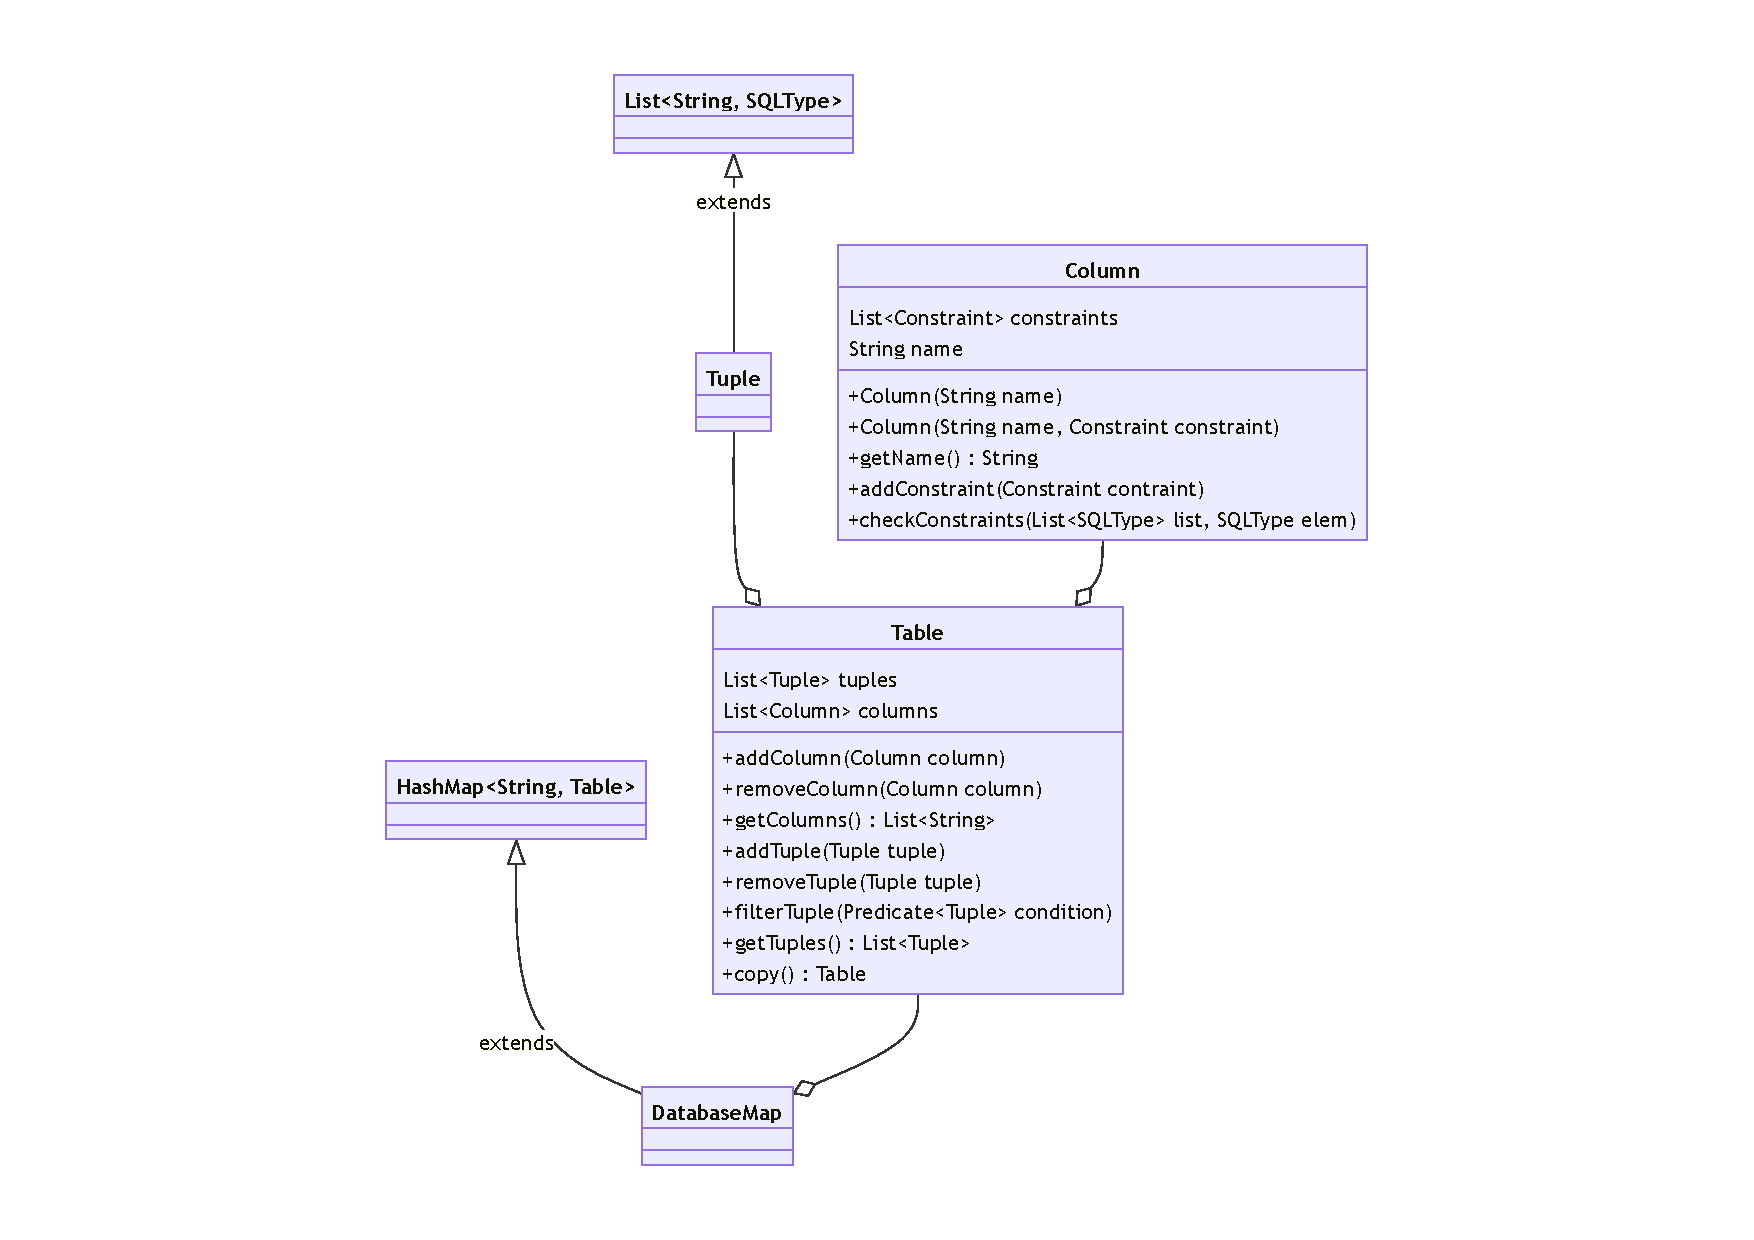
\includegraphics[width=.6\linewidth]{figures/model-diagram.pdf}
    \caption{Schema UML dell'analisi del problema, al suo interno sono rappresentate le entità principali coinvolte nella memorizzazione 
            dei dati e le relazioni tra di esse.}
    \label{fig:model-diagram}
\end{figure}

%----------------------------------------------------------------------------------------
\chapter{Design e Implementazione}
\label{chap:Imple}
%----------------------------------------------------------------------------------------


%----------------------------------------------------------------------------------------
\chapter{Validazione e Conclusioni}
\label{chap:conclusioni}
%----------------------------------------------------------------------------------------


%----------------------------------------------------------------------------------------
% BIBLIOGRAPHY
%----------------------------------------------------------------------------------------

\backmatter

\bibliographystyle{alpha}
\bibliography{bibliography}

%\begin{acknowledgements} % this is optional
%Optional. Max 1 page.
%\end{acknowledgements}

\end{document}
